%%%%%%%%%%%%%%%%%%%%%%%%%BORRAR
\documentclass[a4paper]{article}
\usepackage[utf8]{inputenc}
\usepackage[spanish, es-tabla]{babel}

\usepackage[a4paper, footnotesep = 1cm, width=18cm, left=2cm, top=2.5cm, height=25cm, textwidth=18cm, textheight=25cm]{geometry}
%\geometry{showframe}

\usepackage{tikz}
\usepackage{amsmath}
\usepackage{amsfonts}
\usepackage{amssymb}
\usepackage{float}
\usepackage{graphicx}
\usepackage{caption}
\usepackage{subcaption}
\usepackage{multicol}
\usepackage{multirow}
\setlength{\doublerulesep}{\arrayrulewidth}
\usepackage{xcolor}

\usepackage{hyperref}
\hypersetup{
    colorlinks=true,
    linkcolor=blue,
    filecolor=magenta,      
    urlcolor=blue,
    citecolor=blue,    
}

\newcommand{\quotes}[1]{``#1''}
\usepackage{array}
\newcolumntype{C}[1]{>{\centering\let\newline\\\arraybackslash\hspace{0pt}}m{#1}}
\usepackage[american]{circuitikz}
\usepackage{fancyhdr}
\usepackage{units} 

\pagestyle{fancy}
\fancyhf{}
\lhead{22.13 Electrónica III}
\rhead{Mechoulam, Lambertucci, Martorell, Londero}
\rfoot{\center \thepage}
\begin{document}
\section{auxiliar}
\tableofcontents
%%%%%%%%%%%%%%%%%%%%%%%%%BORRAR

\subsection{Introducción}
\subsubsection{Contadores}
		Los contadores son dispositivos digitales capaces de almacenar la cantidad de pulsos que este recibe. Como todo almacenamiento digital requiere de memoria, los contadores están generalmente constituidos por varias celdas de almacenamiento de 1 bit, comúnmente usados los JK flip-flops. Se puede contemplar la implementación de un JK flip-flip en la Figura (\ref{circ:fkflipflop}) utilizando solamente compuertas lógicas discretas. 
		
		\begin{figure}[H]
	\hspace*{-1cm}
	\centering
	\scalebox{0.7}{
	\begin{circuitikz}
		\draw	
	
			%%%%%%%%%%%%%%%%%%%%%%%%%%%%%
			%FIGURAS
			%%%%%%%%%%%%%%%%%%%%%%%%%%%%%
			
			node[nor port](nor1){} %NOR1
				to[open] ++ (0, -2)
			node[nor port](nor2){} %NOR2
			
			(nor1.in 1) to[open] ++ (-2, 0)
			node[and port, number inputs = 3](and1){} %AND1
			
			(nor2.in 2) to[open] ++ (-2, 0)
			node[and port, number inputs = 3](and2){} %AND2
			
			%%%%%%%%%%%%%%%%%%%%%%%%%%%%%	
	
			(nor1.out) to[short, -*] ++ (0.5, 0)
					node[](feedback1){}
				to[short] ++ (0.5, 0)
				to[short, -*] ++ (0.5, 0)
					node[](feedback2){}
				to[short, -o] ++ (0.5, 0)
				node[label=east:$Q$]{}
			
			(nor2.out) to[short, -*] ++ (0.5, 0)
					node[](feedback3){}
				to[short, -*] ++ (0.5, 0)
					node[](feedback4){}
				to[short] ++ (0.5, 0)
				to[short, -o] ++ (0.5, 0)
				node[label=east:$\overline{Q}$]{}
				
			(feedback1) to[short] ++ (0, -0.38)
				to[short] ++ (-3, -1)
				to[short] ++ (0, -0.3)
				|- (nor2.in 1)
				
			(feedback3) to[short] ++ (0, 0.38)
				to[short] ++ (-3, 1)
				to[short] ++ (0, 0.3)
				|- (nor1.in 2)
				
			(nor1.in 1) -- (and1.out)
			(nor2.in 2) -- (and2.out)
			
			(and1.in 2) to[short, -o] ++ (-1, 0)
				node[label=west:$J$]{}
			
			(and2.in 2) to[short, -o] ++ (-1, 0)
				node[label=west:$K$]{}
				
			(and1.in 3) to[short] ++ (-0.5, 0)
				to[short, -*] ++ (0, -0.922)
				node[](enable){}
				|- (and2.in 1)
				
			(and2.in 3)	to[short] ++ (-0.5, 0)
				|- ++ (6, -0.5)
				-| (feedback2.center)
				
			(and1.in 1) to[short] ++ (-0.5, 0)
				|- ++ (5.5, 0.6)
				-| (feedback4.center)
				
			(enable) to[short] ++ (-0.5, 0)
				to[twoport, -o, l_=Edge Det] ++ (-3, 0)
				node[label=west:$CLK$]{}
	
		;
	\end{circuitikz}
	}
	\caption{Implementación de un JK flip-flop con una totalidad de 8 compuertas lógicas discretas (teniendo en cuenta la implementación de las compuertas AND de tres entradas junto a la corrección de delay.}
	\label{circ:fkflipflop}
\end{figure}
		
		La cantidad de flip-flops necesaria para construir un contador está ligada al mayor número que el dispositivo puede almacenar. Si se quiere contar hasta el número $N$, el contador tendrá que disponer como mínimo de $\lceil log_2(N) \rceil$ flip-flops. Existen dos tipos de contadores: asíncronos y síncronos.
		
\subsubsection{Contadores Asíncronos}
		Los contadores asíncronos poseen un único flip-flop cuya entrada esté conectada al generador de pulsos, propagándose la información provista por este a través del resto para aumentar el contador. Es por esta razón que a los contadores asíncronos se los suele denominar también como contadores por propagación o \textit{ripple counters} en inglés. 

\begin{figure}[H]
	\centering
	\begin{circuitikz}
		\draw
			node[ocirc, label=west:$CLK$]{}
				to[short] ++ (1, 0)
				to[open] ++ (2, 1)
				node[fourport](1){}
				to[open] ++ (3, 0)
				node[fourport](2){}
				to[open] ++ (3, 0)
				node[fourport](3){}
				to[open] ++ (3, 0)
				node[fourport](4){}
				to[open] ++ (-11, -1)
				|- (1.1)
				(1.2) -- (2.1)
				(2.2) -- (3.1)
				(3.2) -- (4.1)
				
				(1.1) ++ (0.13,0) node[]{\scalebox{1.2}{\rotatebox{-90}{$\triangle$}}}
				(2.1) ++ (0.13,0) node[]{\scalebox{1.2}{\rotatebox{-90}{$\triangle$}}}
				(3.1) ++ (0.13,0) node[]{\scalebox{1.2}{\rotatebox{-90}{$\triangle$}}}
				(4.1) ++ (0.13,0) node[]{\scalebox{1.2}{\rotatebox{-90}{$\triangle$}}}
		;
	\end{circuitikz}
	\caption{Conección entre flip-flops para un contador asíncrono.}
	\label{circ:async_counter_connection}		
\end{figure}				
		
		Como los pulsos deben de propagarse a lo largo de varias compuertas lógicas, sucede que para cada incremento en el contador, no todos los bits de la palabra almacenada cambian al mismo instante. En la Figura (\ref{async_ripple}) se esquematiza este efecto para un contador que transita de almacenar un $0111_2$ a almacenar un $1000_2$.

\begin{figure}[H]
	\centering
	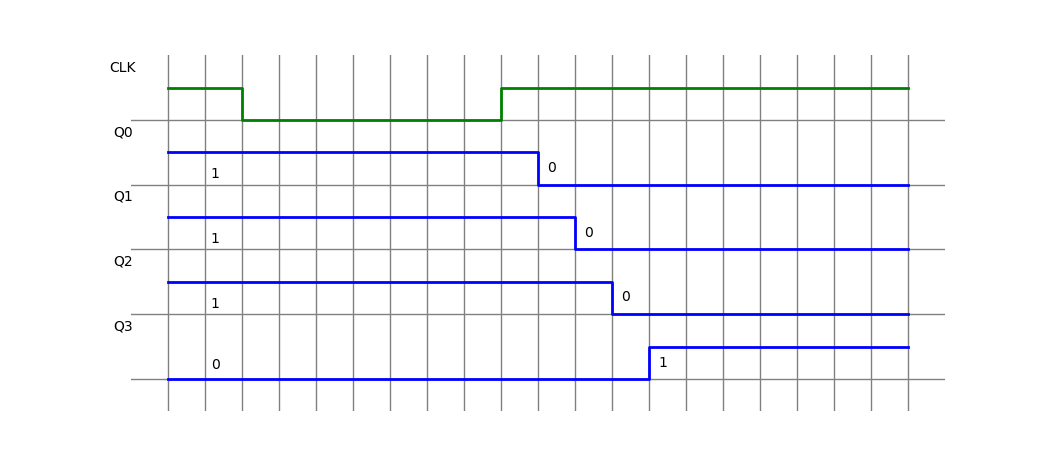
\includegraphics[width=0.7\textwidth]{Imagenes/async_ripple.png}
	\caption{Propagación de un pulso recibido a través de un contador asíncrono para la palabra almacenada transitando del estado $(7)_{10}$ al estado $(8)_{10}$.}
	\label{async_ripple}
\end{figure}

Debido a este fenómeno, las implementaciones asíncronas de contadores no son del todo fidedignas. Sin embargo, abundan como divisores de frecuencia ya que la salida de cada flip-flop será la frecuencia de los pulsos de entrada dividida por una potencia de dos. Otra desventaja de los contadores asíncronos está directamente relacionada con la anterior y es que debido al fenómeno de propagación estos dispositivos se vuelven mucho más lentos en comparación a otros tipos de contadores.

No obstante, la ventaja de esta implementación es que estos dispositivos son muy simples y fáciles de contruir.

\subsubsection{Contadores Síncronos}

\begin{figure}[H]
	\centering
	\begin{circuitikz}
		\draw
			node[ocirc, label=west:$CLK$]{}
				to[short] ++ (1, 0)
					node[](hola){}
				to[open] ++ (2, 1.5)
				node[fourport](1){}
				to[open] ++ (3, 0)
				node[fourport](2){}
				to[open] ++ (3, 0)
				node[fourport](3){}
				to[open] ++ (3, 0)
				node[fourport](4){}
				to[open] ++ (-11, -1)

				(1.1) to[short] ++ (-0.5,0)
					to[short, -*] ++ (0, -1.05)
				(2.1) to[short] ++ (-0.5,0)
					to[short, -*] ++ (0, -1.05)
				(3.1) to[short] ++ (-0.5,0)
					to[short, -*] ++ (0, -1.05)
				(4.1) to[short] ++ (-0.5,0)
					to[short] ++ (0, -1.05)
					to[short] (hola)
				
				
				
				(1.1) ++ (0.13,0) node[]{\scalebox{1.2}{\rotatebox{-90}{$\triangle$}}}
				(2.1) ++ (0.13,0) node[]{\scalebox{1.2}{\rotatebox{-90}{$\triangle$}}}
				(3.1) ++ (0.13,0) node[]{\scalebox{1.2}{\rotatebox{-90}{$\triangle$}}}
				(4.1) ++ (0.13,0) node[]{\scalebox{1.2}{\rotatebox{-90}{$\triangle$}}}
		;
	\end{circuitikz}
	\caption{Conección entre flip-flops para un contador síncrono.}
	\label{circ:sync_counter_connection}		
\end{figure}	

\end{document}